In this research, weather data are an essential element. The main interest of most TOU papers has been to measure how consumers respond to TOU prices or the heterogeneity in their responsiveness across different information stimuli. And the studies have focused on aggregate electricity consumption, consisting of consumption for a wide range of end-use types. Hence, those studies usually do not control temperature variations directly. For example, \cite{The-Effect-of-Information-on-TOU-Electricity-Use:An-Irish-Residential-Study_Pon_2017} and \cite{Peaking-Interest:How-Awareness-Drives-the-Effectiveness-of-Time-of-Use-Electricity-Pricing_Prest_2020}, which also exploited the CER experiment dataset, added weak-of-sample and month-by-year fixed effects (FEs) to their specifications, respectively, in order to control for variations in electricity usage due to seasonal changes. On the other hand, a novel approach adopted in this paper is to decompose household electricity consumption into two broad categories: non-temperature-control- and temperature-control-associated electricity consumption.\footnote{Details of the approach are discussed in Section \ref{Sub-subsection:Breakdown-of-Household-Responses-in-and-near-the-Peak-Rate-Period}.} Since the electricity consumption for temperature-control use is significantly driven by weather, particularly temperatures, it is necessary to link the 30-minute interval consumption data with reliable weather data that is of an appropriate level of resolution. 

\afterpage{
    \begin{figure}[t!]
        \centering
        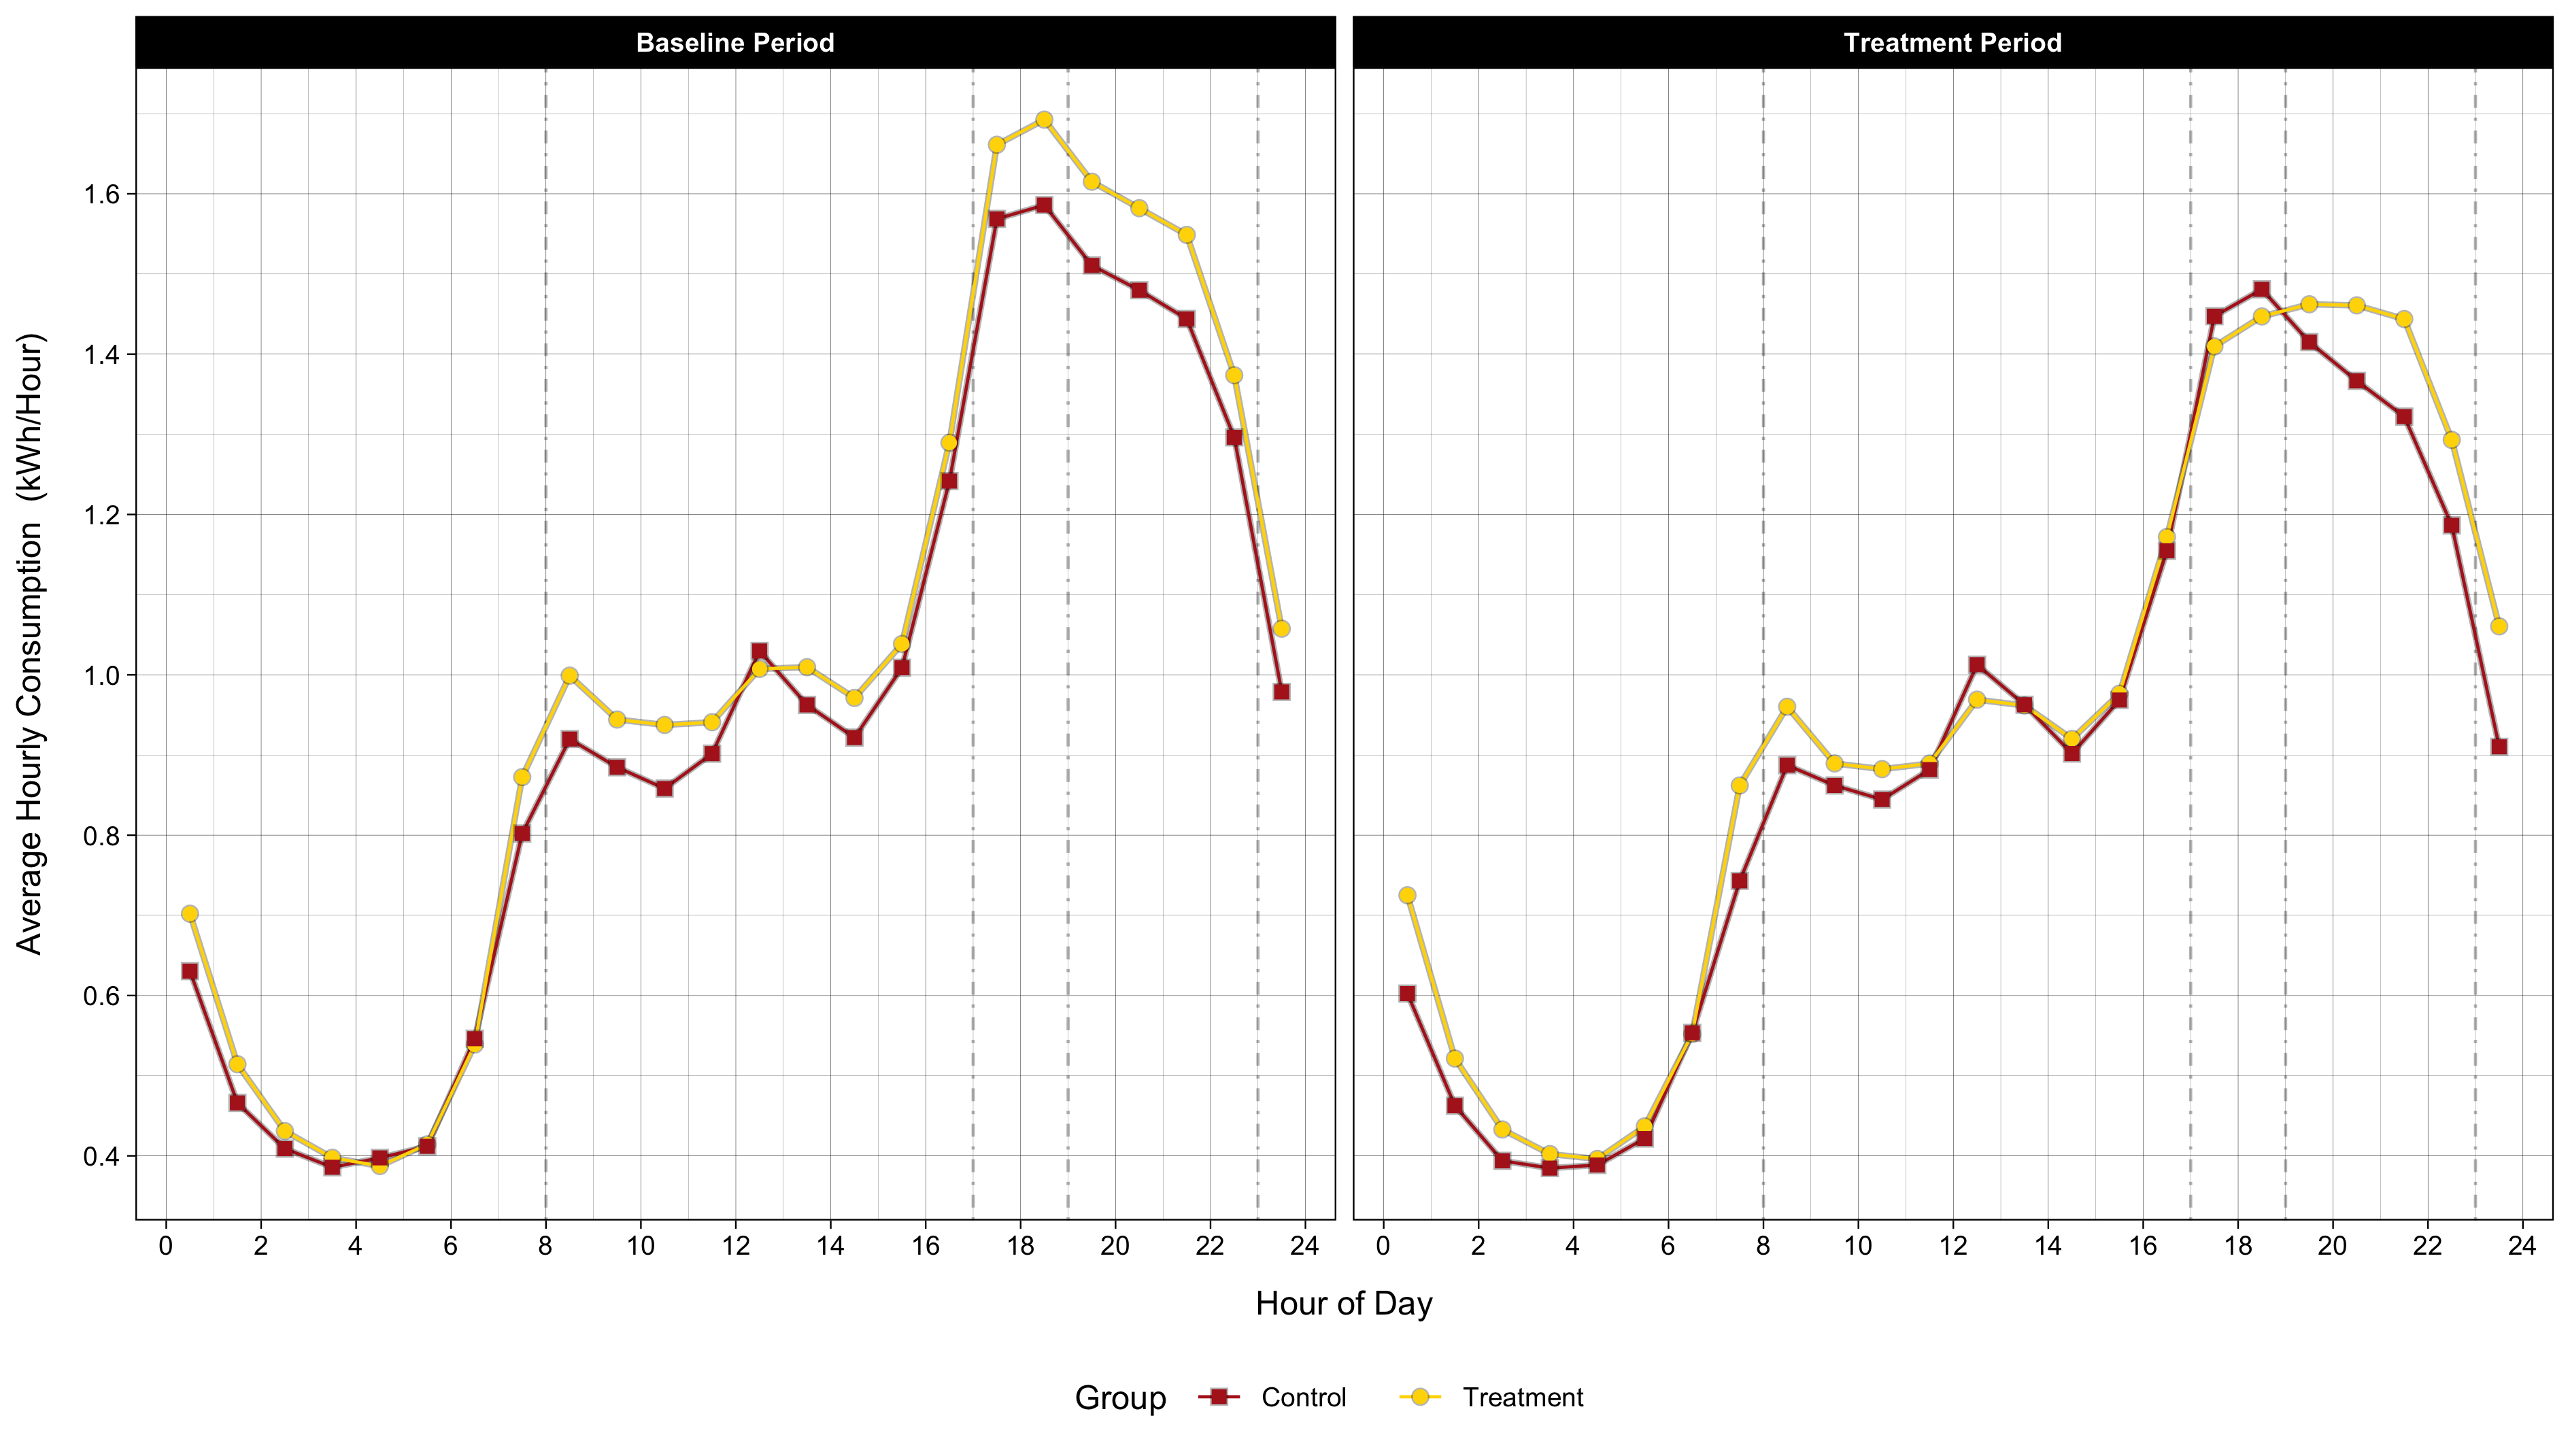
\includegraphics[scale = 0.12]{03_Chapter-2/00A_Figures/Figure_Average-Electricity-Consumption_Within-Day-Average-Hourly-Consumption.png}
        \caption{Average Hourly Electricity Consumption by Time of Day}
        \caption*{
            {\small
            \textit{Note}: The figure shows, during each experiment period, household average hourly electricity consumption for the control and treatment groups, respectively. In general, during the baseline period, households assigned to the treatment group consumed more electricity at a given hour of the day. Although both groups reduced their electricity consumption during the treatment period, the reduction in electricity consumption for the treatment group was much more remarkable for the treatment group than for the control group.
        }}
        \label{Figure:Average-Hourly-Electricity-Consumption-by-Time-of-Day}
    \end{figure}
}
I utilize average daily temperatures in my empirical analysis. More granular temperatures, like hourly temperatures, are not a dominant determinant of temperature-control-driven electricity consumption at a point in time. It is not easy to believe that households adjust their electricity consumption according to ever-changing outside temperatures elaborately and instantly.\footnote{Refer to \textit{3.4 Household Response to Dynamic Prices Exhibits Nontrivial Costs of Action That Impede Peak Reductions} in \cite{Household-Responses-to-Time-Varying-Electricity-Prices_Harding-and-Sexton_2017}.} Furthermore, as shown in Figure \ref{Figure:Average-Hourly-Electricity-Consumption-by-Time-of-Day}, their electricity demand is the lowest in the early morning, the coldest time of the day. Considering those two points, I measure the TOU-tariff-induced reductions in electricity consumption conditional on the average heating needs on a given calendar day. 

I exploit hourly temperature data for the Dublin airport weather station, provided by Met \'{E}ireann, Ireland's National Meteorological Service, to compute average daily temperatures. There is no available location information in the published CER experiment dataset for privacy and security reasons. Therefore, it is impossible to match a participant's consumption data with the weather data of the closest weather monitoring station to him. But fortunately, in Ireland, temperatures do not vary much across areas for a given day. Because of this, I use the mean daily temperatures obtained by averaging the Dublin airport station's hourly temperatures as the representative temperatures in the following analysis. 

Using the average daily temperatures, I calculate daily Heating Degree Days (HDDs). Instead of 65 degrees of Fahrenheit ($^{\circ}F$), a normal base temperature in the United States, 60$^{\circ}F$ is utilized to compute daily HDDs, according to \cite{The-Impacts-of-Climate-Change-on-Domestic-Natural-Gas-Consumption-in-the-Greater-Dublin-Region_Liu-and-Sweeney_2012}. The evolving pattern of temperature-control-driven demand for electricity on days with extreme temperatures could be significantly different under distinct rate structures---e.g., flat and TOU rates. If this is true, the lack of counterfactual consumption observations will cause bias in the measured impact of introducing TOU pricing on household electricity consumption. So, I drop observations for those days in the treatment period when constructing the sample to address the potential threat to the identification. 
